\beginsong{Karussell}[
    wuw={tørtle (Laura Pareigis), VCP Schleswig-Holstein}, 
    jahr={2017}
]

% FIXME: Transcribe notes into proper vector-pdf
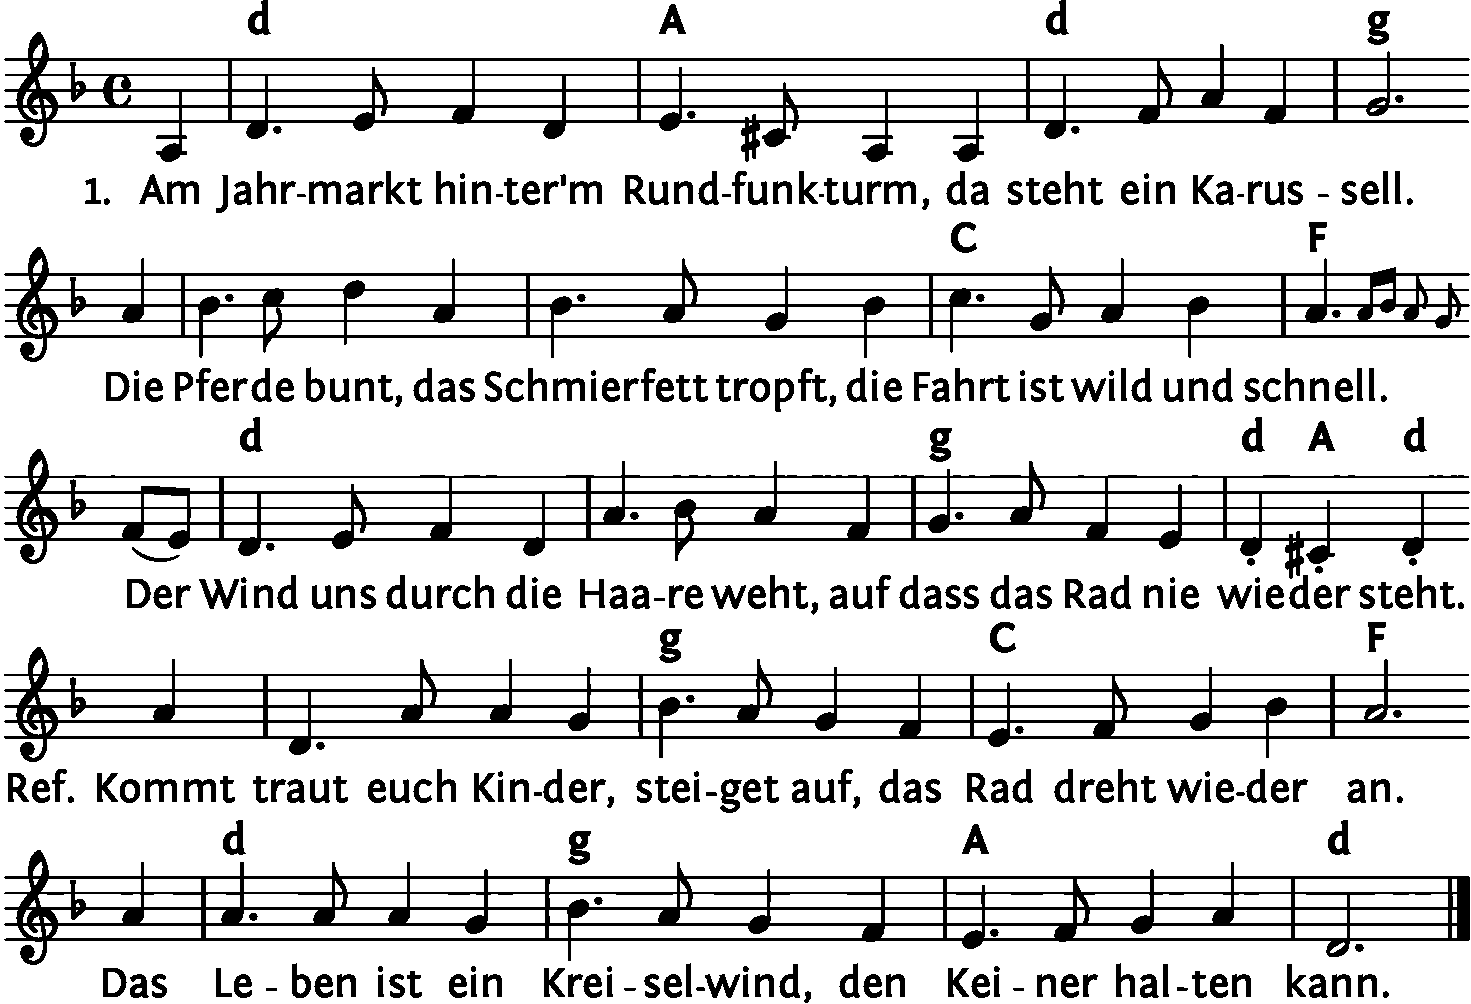
\includegraphics[width=\textwidth, page=1, draft=false]{Noten/Karussell1}

\beginverse
Mein \[D]Pferdchen reißt die \[A7]Hufe hoch,
die \[d]Funken sprühen \[G]weiß,
reißt mir die Zügel aus der Hand
und \[C]bricht dann aus dem \[F]Kreis.
In \[D]Freiheit rennt mein Pferdchen fort
mit \[G]mir an einen \[D]and\[A]er'n \[D]Ort.
Kommt traut euch…
\endverse

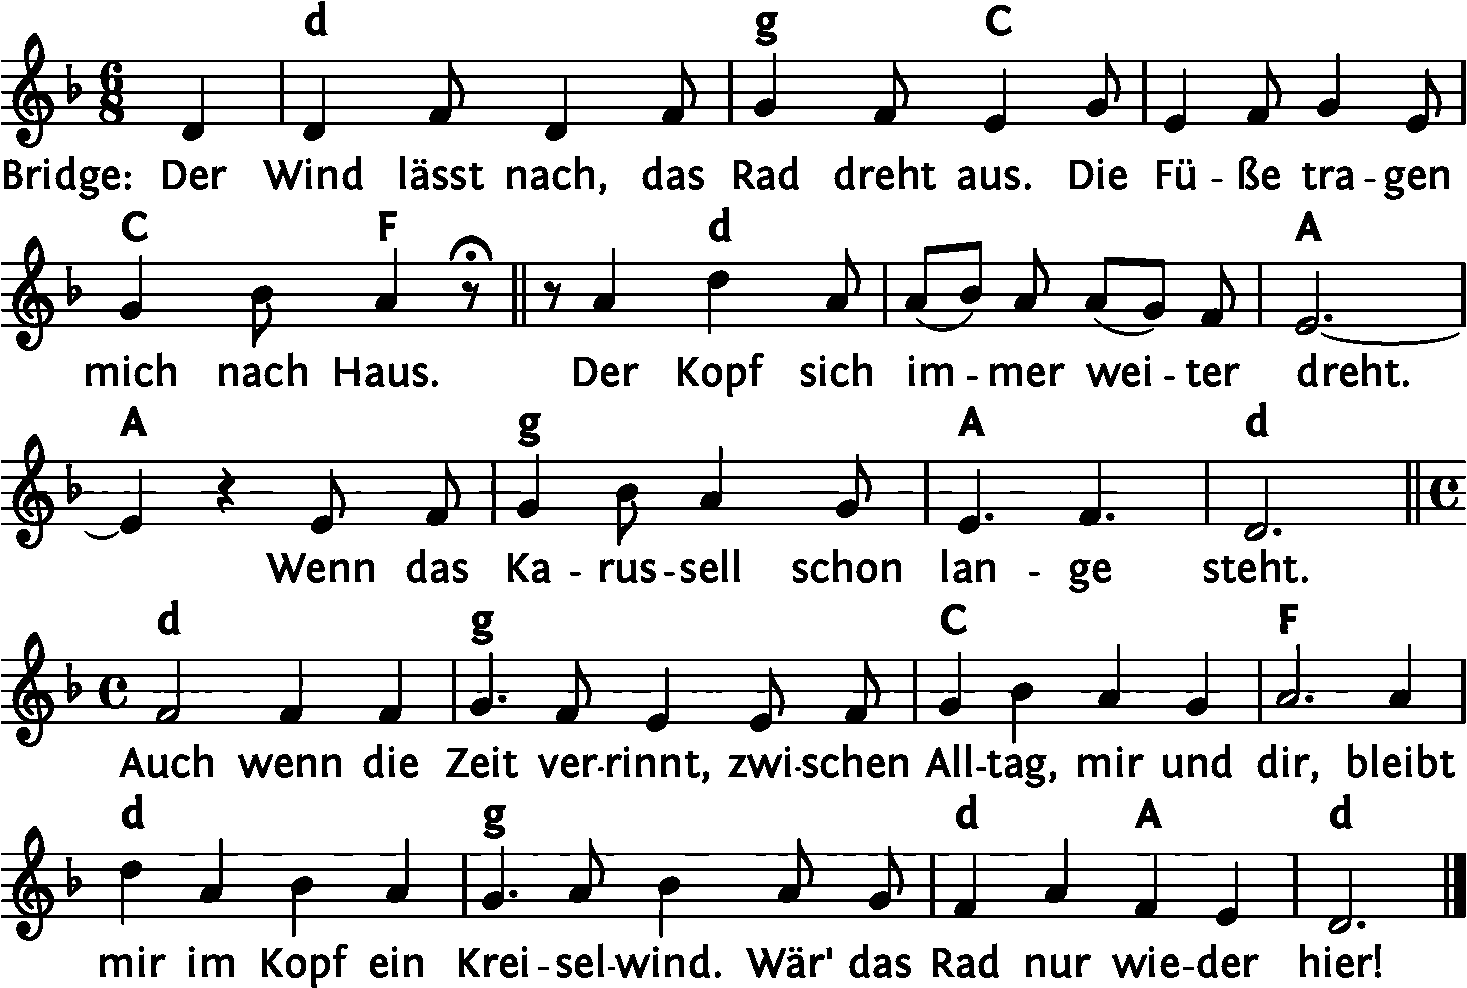
\includegraphics[width=\textwidth, page=1, draft=false]{Noten/Karussell2}

\beginverse
Am \[D]Jahrmarkt hinter'm \[A7]Filmpalast
dreh'n \[D]wir uns wild im \[G]Kreis.
Der Kreiselwind fegt uns durch's Haar
und \[C]jeder von uns \[F]weiß,
dass, \[D]wenn man nachts nach Hause geht,
das \[G]Rad im Kopf nie \[D]wie\[A]der \[D]steht.
Kommt traut euch…
\endverse

\endsong